\section{Appendix}

\subsection{Figures}
\begin{figure}[!h]
    \centering
    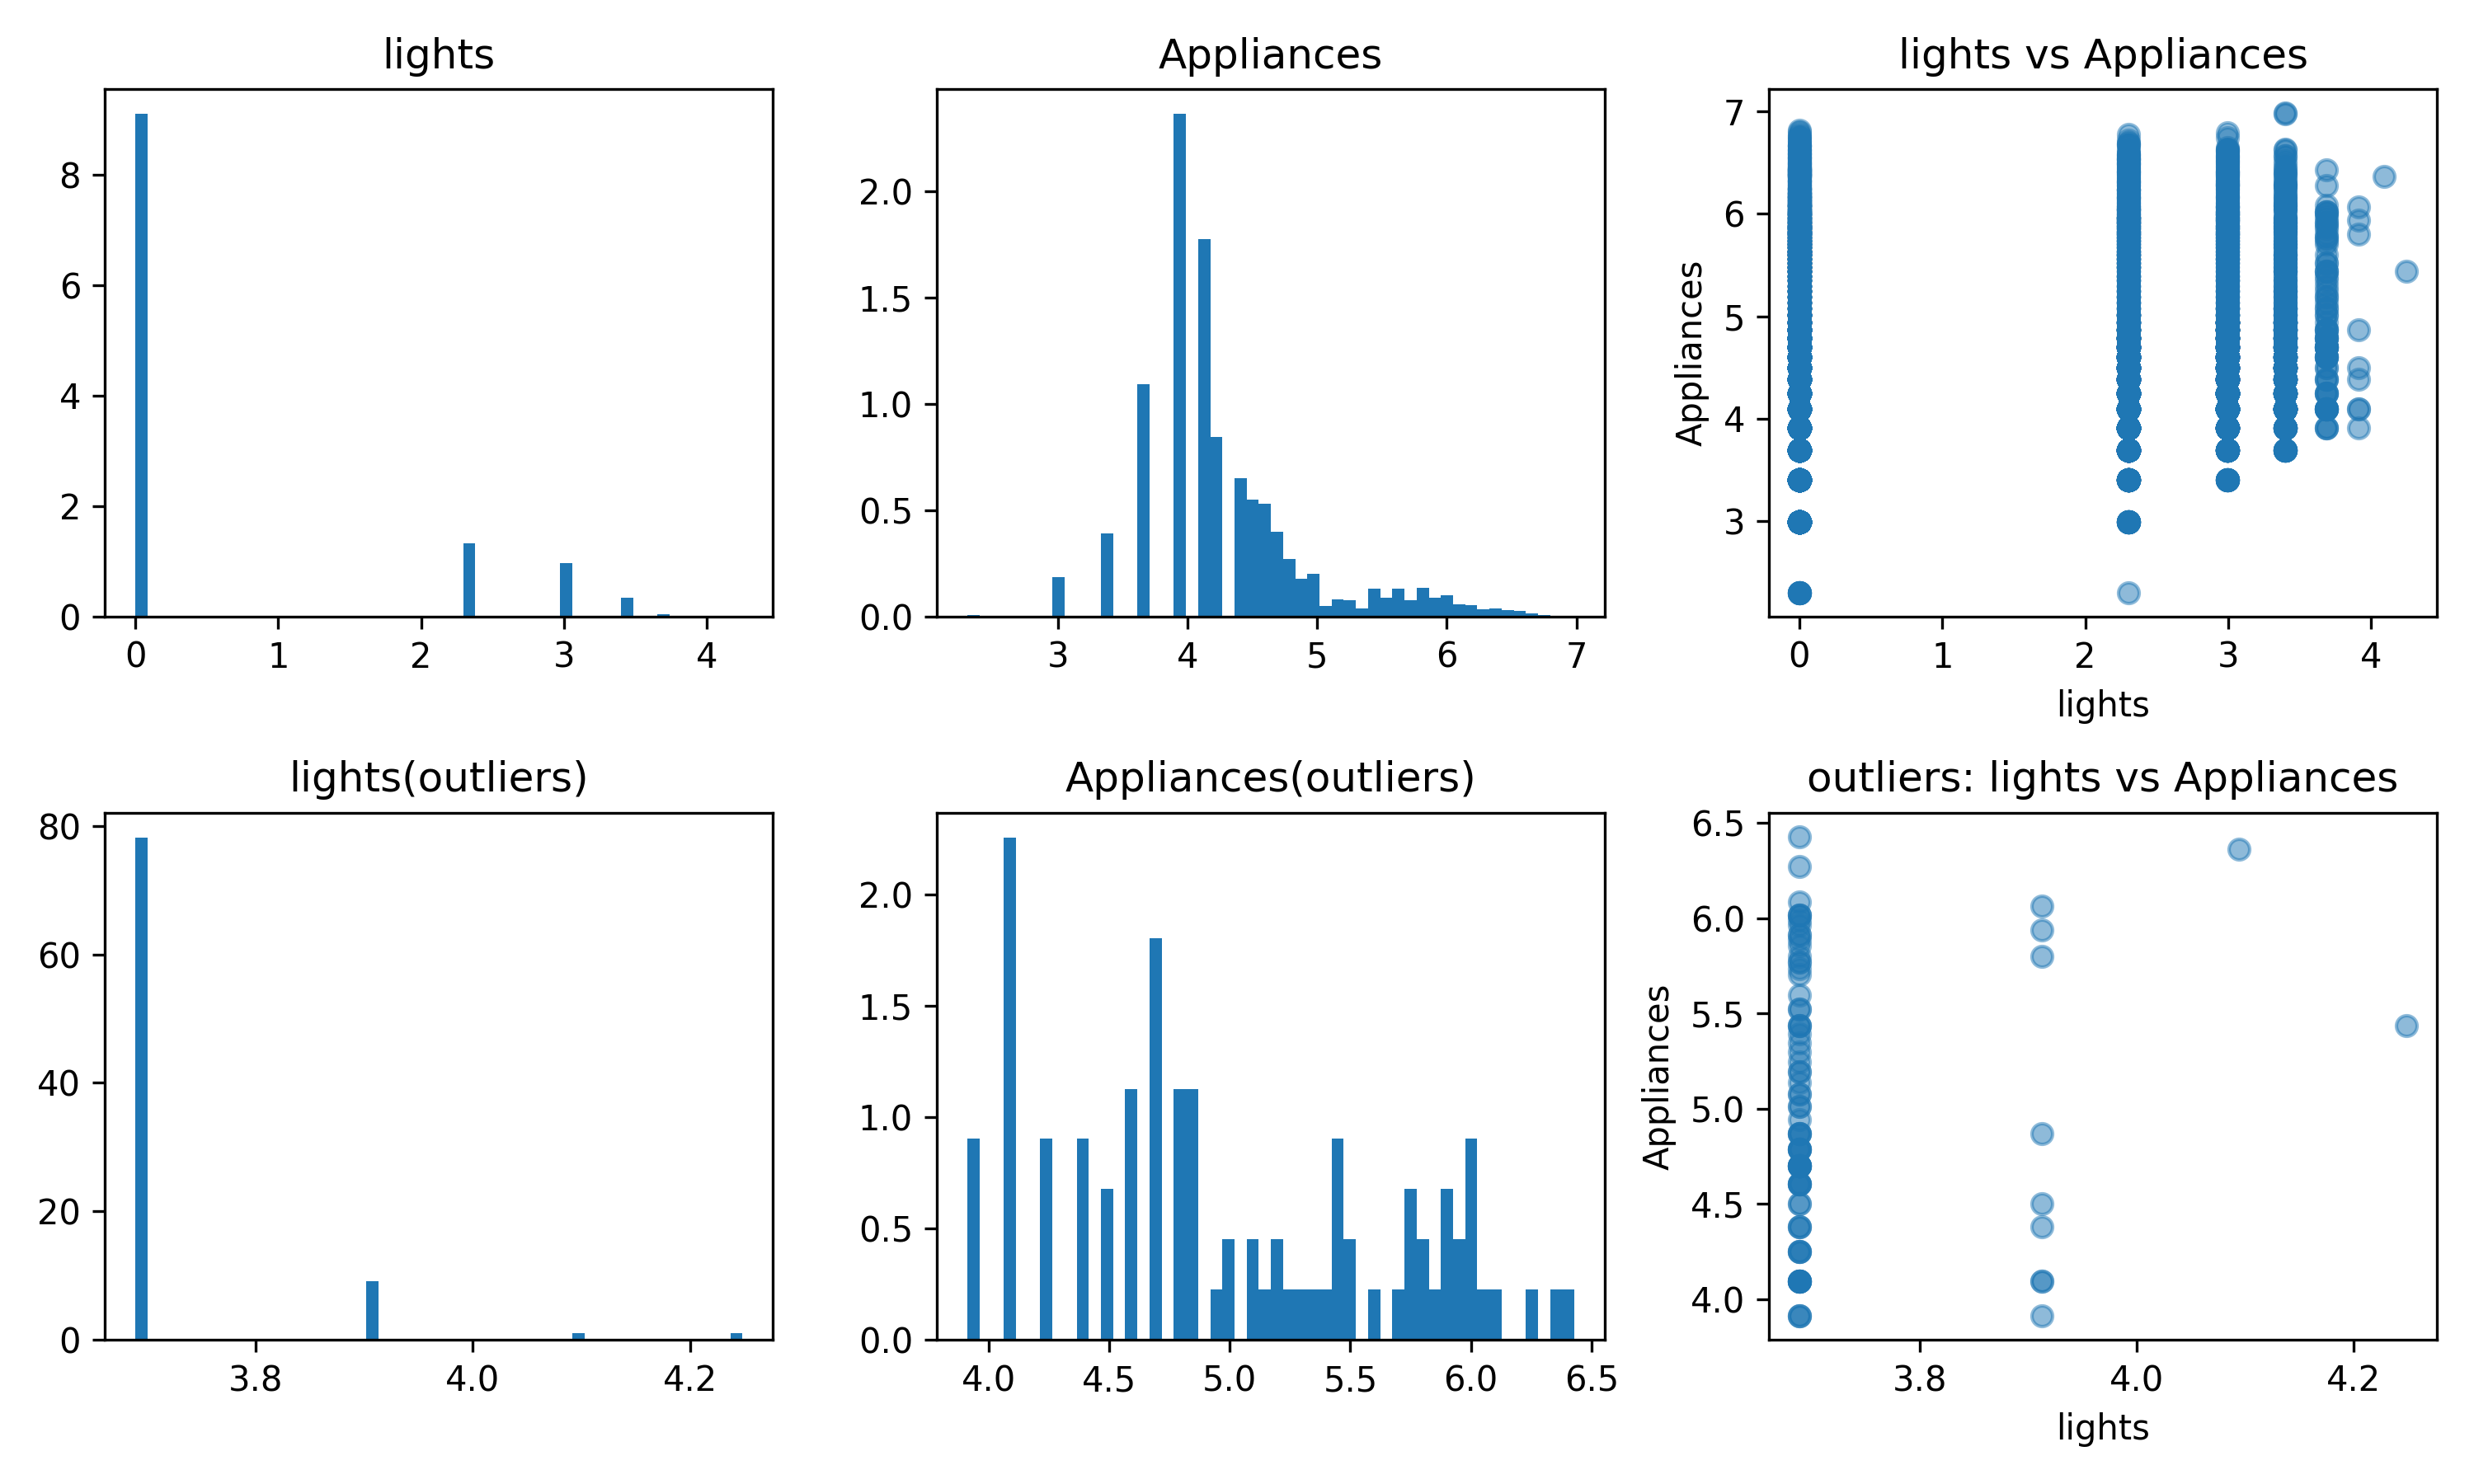
\includegraphics[width=0.9\textwidth]{../results/detect_outliers.png}
    \caption{Distribution of features before and after removing outliers}
\label{fig:skewness}
\end{figure}

\begin{figure}[!h]
    \centering
    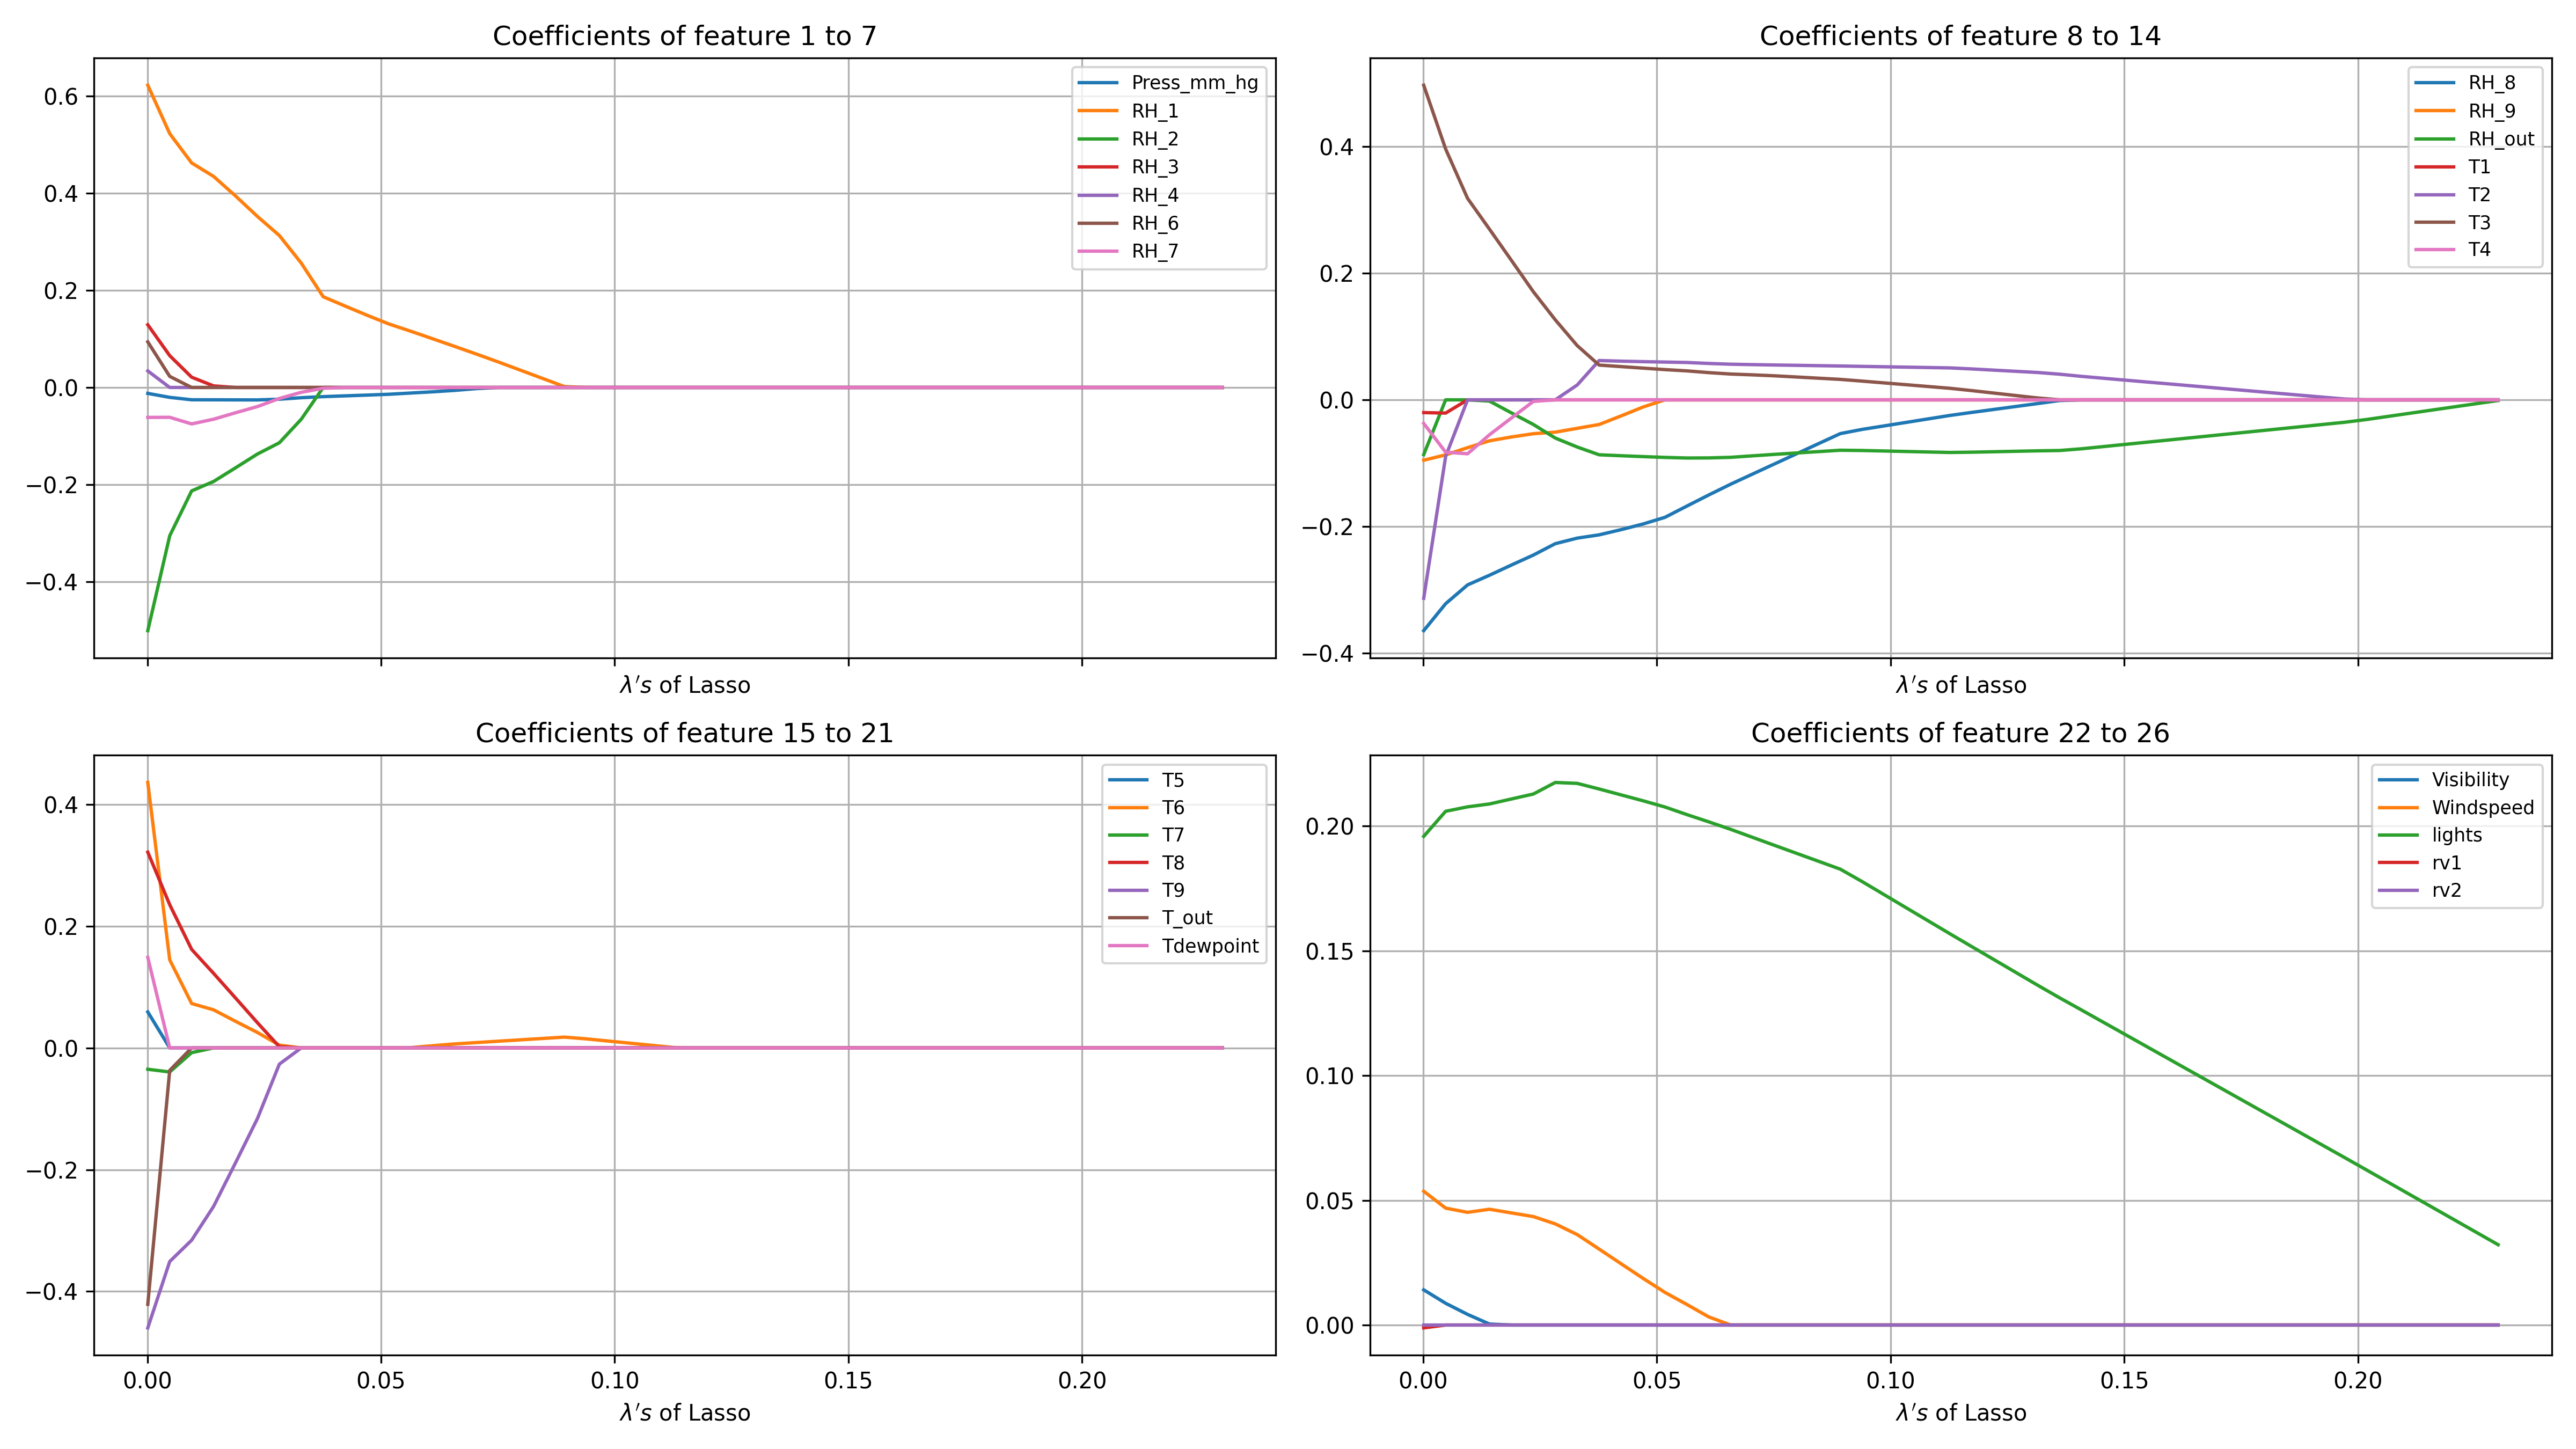
\includegraphics[width=0.9\textwidth]{../results/lasso_select.png}
    \caption{Feature selection using Lasso regression}
    \label{fig:lasso}
\end{figure}

\newpage
\subsection{Table}
\begin{center}
\begin{table}[!h]
    \centering
    \caption{OLS Regression Results}
    \label{tab:linear_regression}
    \begin{tabular}{lclc}
    \toprule
    \textbf{Dep. Variable:}    &    Appliances    & \textbf{  R-squared:         } &     0.268   \\
    \textbf{Model:}            &       OLS        & \textbf{  Adj. R-squared:    } &     0.267   \\
    \textbf{Method:}           &  Least Squares   & \textbf{  F-statistic:       } &     288.0   \\
    \textbf{Date:}             & Mon, 07 Apr 2025 & \textbf{  Prob (F-statistic):} &     0.00    \\
    \textbf{Time:}             &     03:17:47     & \textbf{  Log-Likelihood:    } &   -13165.   \\
    \textbf{No. Observations:} &       15717      & \textbf{  AIC:               } & 2.637e+04   \\
    \textbf{Df Residuals:}     &       15696      & \textbf{  BIC:               } & 2.653e+04   \\
    \textbf{Df Model:}         &          20      & \textbf{                     } &             \\
    \textbf{Covariance Type:}  &    nonrobust     & \textbf{                     } &             \\
    \bottomrule
    \end{tabular}
    \begin{tabular}{lcccccc}
                           & \textbf{coef} & \textbf{std err} & \textbf{t} & \textbf{P$> |$t$|$} & \textbf{[0.025} & \textbf{0.975]}  \\
    \midrule
    \textbf{const}         &       4.8865  &        0.595     &     8.210  &         0.000        &        3.720    &        6.053     \\
    \textbf{Press\_mm\_hg} &      -0.0021  &        0.001     &    -2.897  &         0.004        &       -0.004    &       -0.001     \\
    \textbf{RH\_1}         &       0.0861  &        0.004     &    24.388  &         0.000        &        0.079    &        0.093     \\
    \textbf{RH\_2}         &      -0.0423  &        0.003     &   -14.670  &         0.000        &       -0.048    &       -0.037     \\
    \textbf{RH\_3}         &       0.0047  &        0.004     &     1.091  &         0.275        &       -0.004    &        0.013     \\
    \textbf{RH\_7}         &      -0.0104  &        0.003     &    -4.056  &         0.000        &       -0.015    &       -0.005     \\
    \textbf{RH\_8}         &      -0.0391  &        0.002     &   -15.976  &         0.000        &       -0.044    &       -0.034     \\
    \textbf{RH\_9}         &      -0.0180  &        0.003     &    -6.682  &         0.000        &       -0.023    &       -0.013     \\
    \textbf{T3}            &       0.1480  &        0.006     &    24.182  &         0.000        &        0.136    &        0.160     \\
    \textbf{T4}            &      -0.0453  &        0.006     &    -7.724  &         0.000        &       -0.057    &       -0.034     \\
    \textbf{T6}            &       0.0113  &        0.002     &     7.277  &         0.000        &        0.008    &        0.014     \\
    \textbf{T7}            &      -0.0265  &        0.009     &    -3.067  &         0.002        &       -0.043    &       -0.010     \\
    \textbf{T8}            &       0.0802  &        0.006     &    12.812  &         0.000        &        0.068    &        0.092     \\
    \textbf{T9}            &      -0.0914  &        0.011     &    -8.077  &         0.000        &       -0.114    &       -0.069     \\
    \textbf{Visibility}    &       0.0005  &        0.000     &     1.177  &         0.239        &       -0.000    &        0.001     \\
    \textbf{Windspeed}     &       0.0076  &        0.002     &     3.468  &         0.001        &        0.003    &        0.012     \\
    \textbf{lights}        &       0.1166  &        0.004     &    27.059  &         0.000        &        0.108    &        0.125     \\
    \textbf{month\_2}      &      -0.1164  &        0.020     &    -5.679  &         0.000        &       -0.157    &       -0.076     \\
    \textbf{month\_3}      &      -0.0997  &        0.029     &    -3.489  &         0.000        &       -0.156    &       -0.044     \\
    \textbf{month\_4}      &      -0.2368  &        0.033     &    -7.149  &         0.000        &       -0.302    &       -0.172     \\
    \textbf{month\_5}      &      -0.3200  &        0.042     &    -7.574  &         0.000        &       -0.403    &       -0.237     \\
    \bottomrule
    \end{tabular}
    \begin{tabular}{lclc}
    \textbf{Omnibus:}       & 3750.717 & \textbf{  Durbin-Watson:     } &    2.003  \\
    \textbf{Prob(Omnibus):} &   0.000  & \textbf{  Jarque-Bera (JB):  } & 9389.739  \\
    \textbf{Skew:}          &   1.309  & \textbf{  Prob(JB):          } &     0.00  \\
    \textbf{Kurtosis:}      &   5.736  & \textbf{  Cond. No.          } & 1.02e+05  \\
    \bottomrule
    \end{tabular}
\end{table}
    %\caption{OLS Regression Results}
    \end{center}
    Notes: \newline
     [1] Standard Errors assume that the covariance matrix of the errors is correctly specified. \newline
     [2] The condition number is large, 1.02e+05. This might indicate that there are \newline
     strong multicollinearity or other numerical problems.

\subsection{Code}


